% SPDX-License-Identifier: CC-BY-SA-4.0
% Author: Matthieu Perrin

\begingroup

\begin{frame}[fragile]{La pile de Treiber}

  \vspace{10mm}
  \begin{onlyenv}<1-2>
    \begin{lstlisting}[gobble=6]
      public class Stack<T> {
        private record Node(T (*\Example<2>{value}*), Node (*\Example<2>{next}*)) {}
        private Node (*\Alert<2>{head}*) = null;
        
        public void push(T value) {
          
          (*\Alert<2>{head =}*) new Node(value, head);
          
        }
        
        public T pop() {
          
          if(head==null) return null;
          T value = head.value();
          (*\Alert<2>{head =}*) head.next();
          return value;
          
        }
      }
    \end{lstlisting}
  \end{onlyenv}
  \begin{onlyenv}<3-4>
    \begin{lstlisting}[gobble=6]
      public class Stack<T> {
        private record Node(T value, Node next) {}
        private (*\Alert<3>{AtomicReference<Node> head}*) = new AtomicReference<>(null);
        
        public void push(T value) {
          
          head.(*\Alert<3>{set}*)(new Node(value, head.(*\Alert{get}*)()));
          
        }
        
        public T pop() {
          
          if(head.(*\Alert{get}*)()==null) return null;
          T value = head.(*\Alert{get}*)().value();
          head.(*\Alert<3>{set}*)(head.(*\Alert{get}*)().next());
          return value;
          
        }
      }
    \end{lstlisting}
  \end{onlyenv}
  \begin{onlyenv}<5-6>
    \begin{lstlisting}[gobble=6]
      public class Stack<T> {
        private record Node(T value, Node next) {}
        private AtomicReference<Node> head = new AtomicReference<>(null);
        
        public void push(T value) {
          (*\Alert<5>{Node old = head.get();}*)
          head.(*\Alert<6>{set}*)(new Node(value, old));
          
        }
        
        public T pop() {
          
          (*\Alert<5>{Node old = head.get();}*)
          if(old==null) return null;
          head.(*\Alert<6>{set}*)(old.next());
          return old.value();
          
        }
      }
    \end{lstlisting}
  \end{onlyenv}
  \begin{onlyenv}<7>
    \begin{lstlisting}[gobble=6]
      public class Stack<T> {
        private record Node(T value, Node next) {}
        private AtomicReference<Node> head = new AtomicReference<>(null);
        
        public void push(T value) {
          (*\Example{do}*) {
            Node old = head.get();
          } while(!head.(*\Alert{compareAndSet}*)(old, new Node(value, old)));
        }
        
        public T pop() {
          (*\Example{for(;;)}*) {
            Node old = head.get();
            if(old==null) return null;
            if(head.(*\Alert{compareAndSet}*)(old, old.next())
            return old.value();
          }
        }
      }
    \end{lstlisting}
  \end{onlyenv}

  \on[top]{
    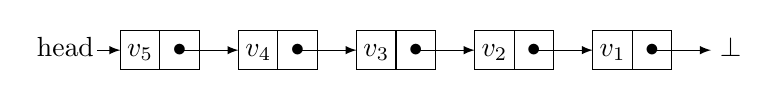
\begin{tikzpicture}[anchor=mid]
      \draw (-.7,.25) node{head};
      \draw[-latex] (-.3,0.25) -- (0,0.25);
      \draw (0.0,0) rectangle +(.5,.5) rectangle +(1,0) +(.25,.25) node{$v_5$} +(.75,.25) node{$\bullet$};
      \draw (1.5,0) rectangle +(.5,.5) rectangle +(1,0) +(.25,.25) node{$v_4$} +(.75,.25) node{$\bullet$};
      \draw (3.0,0) rectangle +(.5,.5) rectangle +(1,0) +(.25,.25) node{$v_3$} +(.75,.25) node{$\bullet$};
      \draw (4.5,0) rectangle +(.5,.5) rectangle +(1,0) +(.25,.25) node{$v_2$} +(.75,.25) node{$\bullet$};
      \draw (6.0,0) rectangle +(.5,.5) rectangle +(1,0) +(.25,.25) node{$v_1$} +(.75,.25) node{$\bullet$};
      \draw[-latex] (0.0,0) +(.75,.25) -- +(1.5,.25);
      \draw[-latex] (1.5,0) +(.75,.25) -- +(1.5,.25);
      \draw[-latex] (3.0,0) +(.75,.25) -- +(1.5,.25);
      \draw[-latex] (4.5,0) +(.75,.25) -- +(1.5,.25);
      \draw[-latex] (6.0,0) +(.75,.25) -- +(1.5,.25);
      \draw (7.5,0) +(.25,.25) node{$\bot$} ;
    \end{tikzpicture}
  }
  
  \onBlock[right=4.5cm, bottom=7mm]{Conseils}{
    \begin{enumerate}
    \item Écrire le code séquentiel
    \item<2-> Identifier les variables
      \begin{itemize}
      \item {\color{exampleColor}constantes}
      \item \alert{mutables}
      \end{itemize}
    \item<4-> Isoler les lectures
    \item<6-> Protéger les écritures
    \end{enumerate}
  }

  \footnoteref{R. Kent Treiber. \textit{Systems programming: Coping with parallelism.} IBM technical report (1986)}
  
\end{frame}

\endgroup
\endinput
